\chapter{Технологический раздел}
\label{cha:impl}
В данном разделе будут представлены средства реализации, разработанные алгоритмы и интерфейс.

\section{Средства реализации}
\label{sec:realisation}
В качестве языка программирования был выбран Python~\cite{python} по скольку это объектно-ориентированный язык, рассматриваемый во время учёбы, что значительно сокращает время написания программы и упрощает разработку.
\par В качестве среды разработки была выбрана "PyCharm Community Edition"\!,  а для представления пользовательского интерфейса библиотека PyQt5~\cite{pyqt}.
\section{Описание структуры программы}
\label{sec:structure}
\paragraph{Описание основных модулей программы}
\begin{itemize}
	\item main.py -- загружает интерфейс и запускает программу;
	\item window.py -- содержит класс интерфейса;
	\item sceneinterface.py -- содержит класс SceneInterface, выступающий в качестве посредника между сценой и интерфейсом;
	\item scene.py -- содержит класс сцены, основной класс, в котором находятся объекты и источники света;
	\item commands.py -- содержит классы команд, которые влияют на сцену;
	\item controlmanager.py -- содержит классы менеджеров, отвечающие за выполнение сложных команд, таких как отрисовка и загрузка моделей;
	\item builder.py -- содержит класс Builder, отвечающий за чтение файла и создание объекта модели;
	\item builddirector.py -- содержит класс, контролирующий создание объекта;
	\item drawer.py -- содержит классы QDrawer и BaseDrawer, которые предоставляют методы отрисовки на самом низком уровне;
	\item drawerfactory.py -- содержит классы DrawerFactory и QDrawerFactory, целью которых является создание объекта Drawer;
	\item baseobject.py -- содержит класс базового объекта, точки и вектора;
	\item invisibleobject.py -- содержит класс камеры и источника света;
	\item visibleobject.py -- содержит класс полигона;
	\item visitor.py -- содержит методы, применяемые к разным объектам сцены, а именно перемещение и поворот;
	\item visualizer.py -- содержит методы, отвечающие за взаимодействие с drawer-ом;
	\item musclemodel.py -- содержит класс эллипсоида, прямой мышцы и сложной мышцы;
\end{itemize}
\par На рисунке \ref{fig:scheme} представлена диаграмма классов, из неё видно разделение на отдельные модули, что позволяет изменять и дополнять некоторые из них независимо от других, благодаря чему программу будет проще обновлять при необходимости.
\begin{figure}[H]
	\centering
	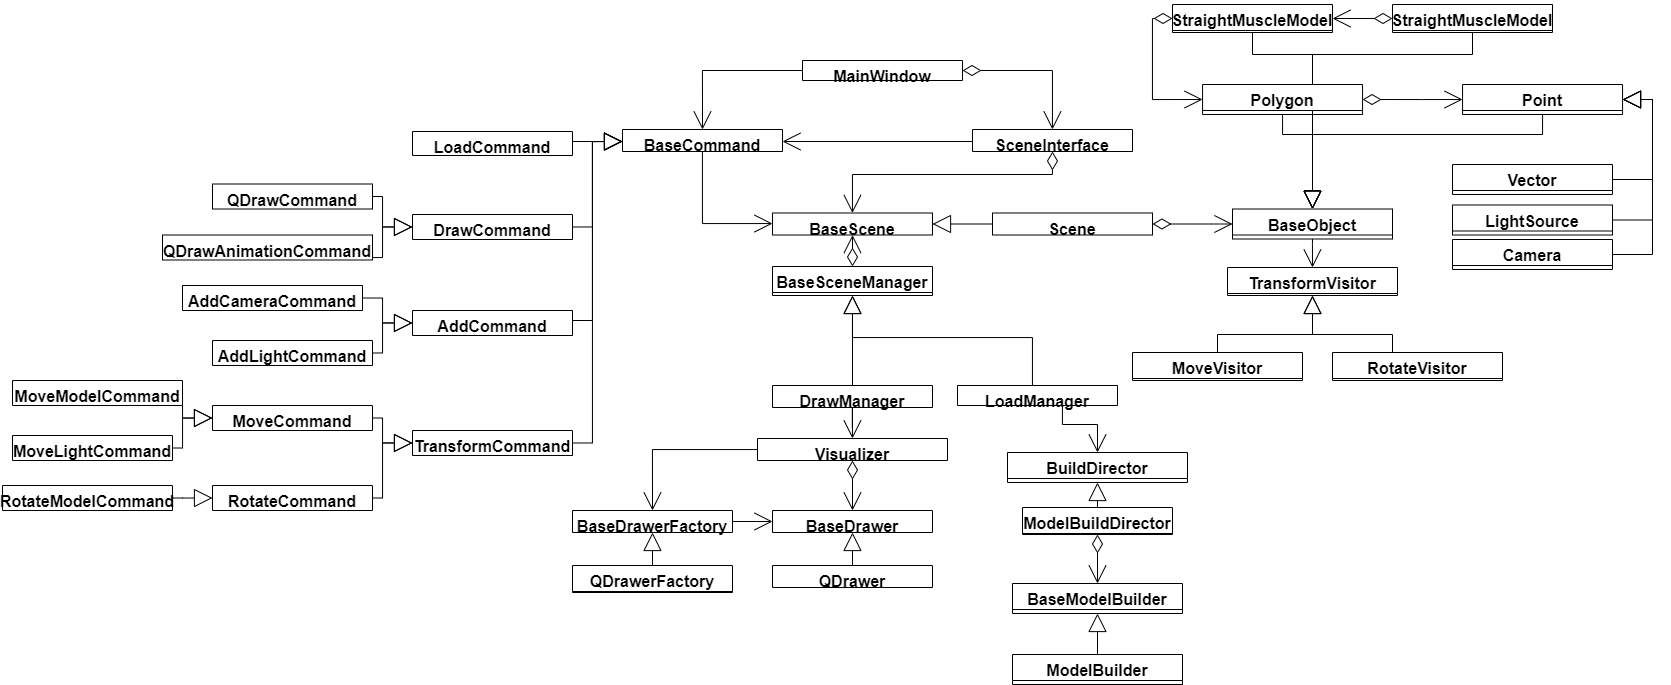
\includegraphics[height=0.35\paperheight, angle=90]{images/scheme}
	\caption{Диаграмма классов}
	\label{fig:scheme}
\end{figure}


\section{Листинг кода}
В листинге \ref{code:zbuf} представлен код класса Z-буффера, который содержит метод \Code{process\_polygon(self, polygon, light)} на вход которого подаётся полигон и массив источников света, а он растеризует поданный треугольник, вызывает метод для вычисления интенсивности цвета полигона и заполняет экранный и z-буфер.
\begin{lstlisting}[caption= Класс Z-буффера, label=code:zbuf]
	class ZBuffer(object):
		def __init__(self, visualizer, width=900, height=900):
			self.width = width
			self.height = height
			self.visualizer = visualizer
			self._buf = [[-6000 for _ in range(width)] for __ in range(height)]
			
		def process_polygon(self, polygon, light):
			color = polygon.get_color(light)
			
			points = polygon.get_points()
			x = [floor(points[i].x) for i in range(3)]
			y = [floor(points[i].y) for i in range(3)]
			
			ymax = min(max(y), self.height)
			ymin = min(min(y), 0)
			
			x1 = x2 = 0
			z1 = z2 = 0
			for y_current in range(ymin, ymax+1):
				first_cycle = 1
				for n in range(3):
					n1 = 0 if n == 2 else n + 1
					if y_current >= max(y[n], y[n1]) or y_current < min(y[n], y[n1]):
						continue
					
					m = float(y[n] - y_current) / (y[n]-y[n1])
					if first_cycle == 0:
						x2 = x[n] + floor(m * (x[n1] - x[n]))
						z2 = points[n].z + m * (points[n1].z - points[n].z)
					else:
						x1 = x[n] + floor(m * (x[n1] - x[n]))
						z1 = points[n].z + m * (points[n1].z - points[n].z)
						
					first_cycle = 0
				
				if x2 < x1:
					x2, x1 = x1, x2
					z2, z1 = z1, z2
					
				x_max = min(x2, self.width)
				x_min = max(x1, 0)
				for x_current in range(x_min, x_max):
					m = float(x1 - x_current) / (x1 - x2)
					z_current = z1 + m * (z2 - z1)
					self.process_point(x_current, y_current, int(z_current), color)
		
		def process_point(self, x: int, y: int, z: int, color):
			if z > self._buf[x][y]:
				self._buf[x][y] = z
				self.visualizer.drawPoint(x, y, color)
\end{lstlisting}
В листинге \ref{code:color} представлен метод вычисления интенсивности цвета полигона по формуле Ламберта. 
\begin{lstlisting}[caption= Метод рассчёта интенсивности цвета полигона, label=code:color]
	def get_color(self, lights):
		x, y, z = 0, 0, 0
		for p in self.get_points():
			xt, yt, zt = p.get_position()
			x += xt
			y += yt
			z += zt
		
		centroid = Point(x / 3, y / 3, z / 3)
		normal = self.get_normal().normalize()
		
		intensity = 0.4
		for light in lights:
			v = Vector().from_points(light, centroid).normalize()
			cos = max(v.scalar_multiplication(normal), 0)
			intensity += light.intensity * cos
			
		rgb = list(QColor(self.color).getRgbF())
		
		rgb[0] *= intensity
		rgb[1] *= intensity
		rgb[2] *= intensity
		
		return QColor().fromRgbF(rgb[0], rgb[1], rgb[2])
\end{lstlisting}

В листинге \ref{code:ellipse} представлен код класса эллипсоида, в котором в методе \Code{\_\_init\_\_(self)} определяются координаты вершин исходного куба, а в методе \Code{rec\_subdivide(self, d)} производится рекурсивное разбиение его полигонов.
\begin{lstlisting}[caption= Класс эллипсоида, label=code:ellipse]
	class Ellipsoid(object):
		def __init__(self):
			x = 1
			z = 1
			y = 1
			
			self.vertex_list = [
			[-x, -y, -z], [x, -y, -z], [x, -y, z], [-x, -y, z],
			[-x, y, -z], [x, y, -z], [x, y, z], [-x, y, z]
			]
			
			self.triangle_list = [
			[0,2,1], [0,3,2], [1,5,0], [5,4,0], [0,4,7], [7,3,0],
			[6,5,1], [1,2,6], [7,2,3], [7,6,2], [4,5,6], [6,7,4]
			]
			
			self.result_ind = []
			self.result_vertexes = []
		
		@staticmethod
		def normalize(v):
			d = sqrt(v[0] * v[0] + v[1] * v[1] + v[2] * v[2])
			if d == 0.0:
				print("zero division")
			v[0] /= d
			v[1] /= d
			v[2] /= d
		
		def start_division(self, d):
			self.result_ind = []
			self.result_vertexes = []
			for i in range(12):
				self.rec_subdivide( self.vertex_list[self.triangle_list[i][0]],
					self.vertex_list[self.triangle_list[i][1]],
					self.vertex_list[self.triangle_list[i][2]], d)
			
			for vertex in self.result_vertexes:
				self.normalize(vertex)
		
		def rec_subdivide(self, v1, v2, v3, d):
			v12 = [0, 0, 0]
			v23 = [0, 0, 0]
			v31 = [0, 0, 0]
			
			if d == 0:
				if v1 not in self.result_vertexes:
					self.result_vertexes.append(v1)
				if v2 not in self.result_vertexes:
					self.result_vertexes.append(v2)
				if v3 not in self.result_vertexes:
					self.result_vertexes.append(v3)
				t = [0, 0, 0]
				t[0] = self.result_vertexes.index(v1)
				t[1] = self.result_vertexes.index(v2)
				t[2] = self.result_vertexes.index(v3)
				
				self.result_ind.append(t)
				return
		
			for i in range(3):
				v12[i] = (v1[i] + v2[i]) / 2
				v23[i] = (v2[i] + v3[i]) / 2
				v31[i] = (v3[i] + v1[i]) / 2
			
			self.rec_subdivide(v1, v12, v31, d - 1)
			self.rec_subdivide(v2, v23, v12, d - 1)
			self.rec_subdivide(v3, v31, v23, d - 1)
			self.rec_subdivide(v12, v23, v31, d - 1)
		
		def reshape(self, x, y, z):
			for vertex in self.result_vertexes:
				vertex[0] *= x
				vertex[1] *= y
				vertex[2] *= z
			
		def polygonise(self, center_x=0, center_y=0, center_z=0):
			polygons = []
			for triangle in self.result_ind:
				p1 = Point(self.result_vertexes[triangle[0]][0] + center_x, self.result_vertexes[triangle[0]][1] + center_y, self.result_vertexes[triangle[0]][2] + center_z)
				p2 = Point(self.result_vertexes[triangle[1]][0] + center_x, self.result_vertexes[triangle[1]][1] + center_y, self.result_vertexes[triangle[1]][2] + center_z)
				p3 = Point(self.result_vertexes[triangle[2]][0] + center_x, self.result_vertexes[triangle[2]][1] + center_y, self.result_vertexes[triangle[2]][2] + center_z)
				polygons.append(Polygon(p1, p2, p3))
			return polygons
\end{lstlisting}

В листинге \ref{code:morph} представлен код класса Morph, который содержит в себе методы, необходимые для вычисления промежуточных мешей, а именно метод установления между начальными и результирующими полигонами \Code{straight\_map(self)} и метод \Code{calculate\_paths(self)}, рассчитывающий путь, который необходимо преодолеть каждой вершине каждого полигона.
\begin{lstlisting}[caption= Класс морфинга, label=code:morph]
	class Morph(object):
		def __init__(self, begin, end, frames=30):
			self.begin = begin
			self.end = end
			self.paths = []
			self.pairs = []
			
			self.frames = frames
			
			self.straight_map()
			self.calculate_paths()
			
		def straight_map(self):
			number = len(self.begin)
			self.pairs = [[i, i, 0] for i in range(number)]
			return self.pairs
		
		def calculate_paths(self):			
			for pair in self.pairs:
				p1 = self.begin[pair[0]].get_points()
				p2 = self.end[pair[1]].get_points()
				v3 = []
				for i in range(3):
					v = Vector()
					v.from_points(p1[i], p2[i])
					v3.append(v)
				
				self.paths.append(v3)
			
			return self.paths
		
		def get_frame(self, frame_number):
			number = len(self.begin)
			result = []
			
			for i in range(number):
				points = self.begin[self.pairs[i][0]].get_points()
				for p in range(3):
					points[p] = points[p] + \ self.paths[self.pairs[i][0]][p]. \ number_multiplication(frame_number) / self.frames
				result.append(Polygon(points[0], points[1], points[2], self.begin[self.pairs[i][0]].color))
			
			return result
\end{lstlisting}

\section{Интерфейс программы}
На рисунке \ref{fig:wholeinterface} представлен интерфейс программы.
\begin{figure}[H]
	\centering
	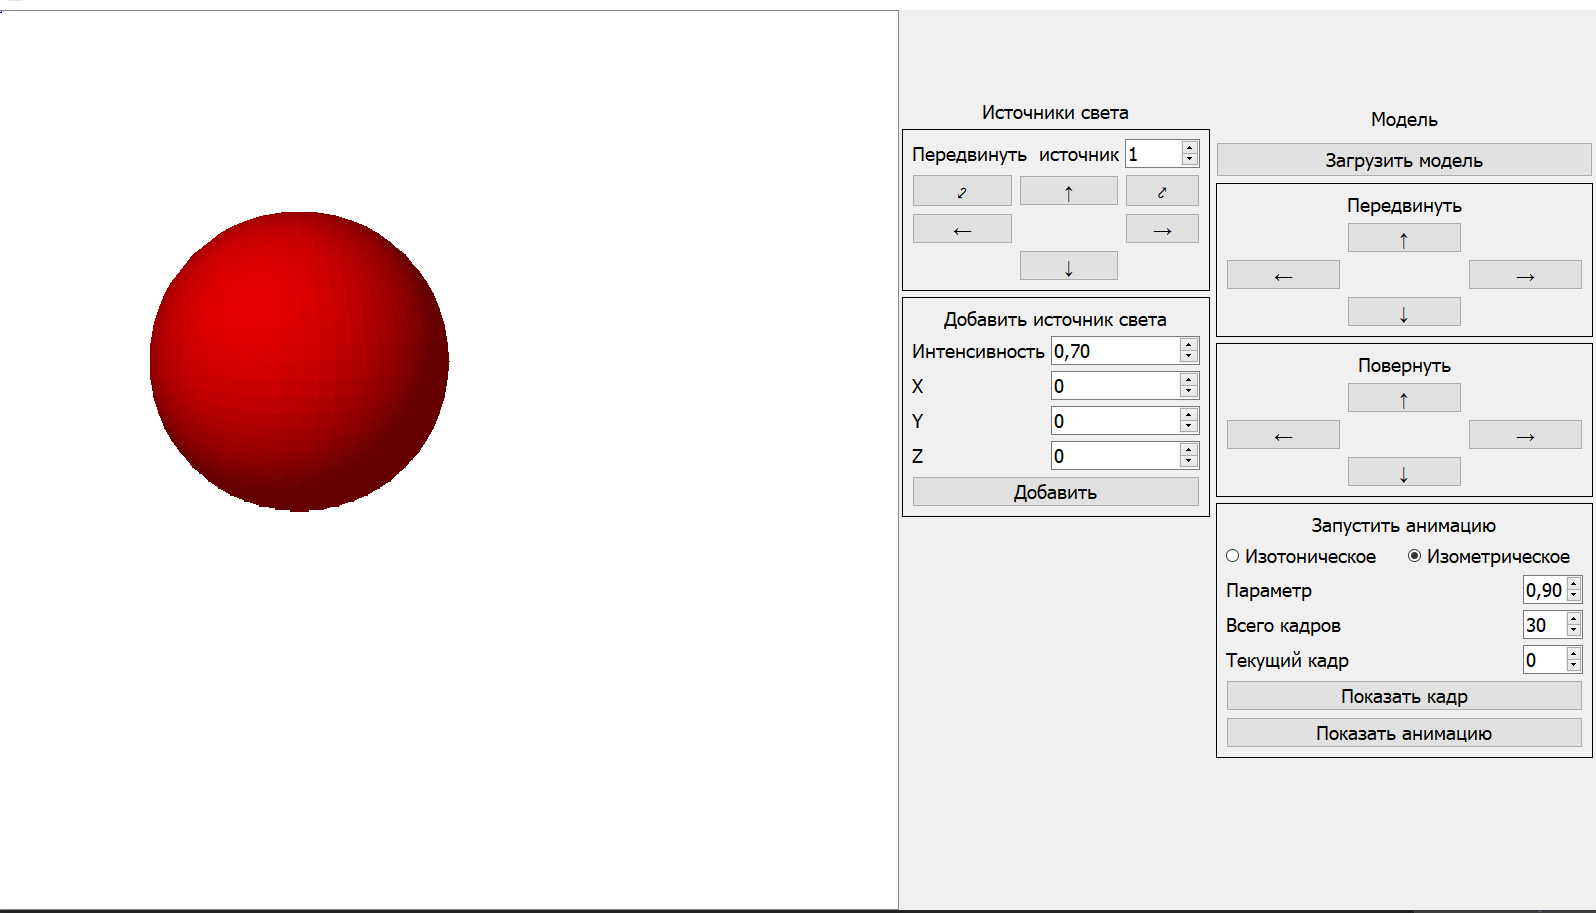
\includegraphics[width=0.9\linewidth]{images/whole_interface}
	\caption{Интерфейс программы}
	\label{fig:wholeinterface}
\end{figure}
Интерфейс включает в себя блок взаимодействия с источниками света и блок взаимодействия с моделью. Первый, представленный на рисунке \ref{fig:lights}, предоставляет возможности:
\begin{itemize}
	\item передвинуть источник света по одной из 3 осей;
	\item добавить новый источник света, задав его интенсивность и координаты.
\end{itemize}
\begin{figure}[H]
	\centering
	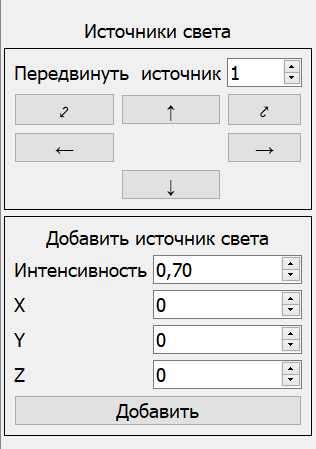
\includegraphics[width=0.4\linewidth]{images/lights}
	\caption{Блок взаимодействия с источниками света}
	\label{fig:lights}
\end{figure}

Второй блок, представленный на рисунке \ref{fig:models}, содержит поля, отвечающие за:
\begin{itemize}
	\item загрузку модели;
	\item перемещение и поворот модели;
	\item выбор типа сокращения -- изометрическое или изотоническое сокращение;
	\item выбор количества кадров анимации;
	\item отображение анимации и отдельных промежуточных кадров.
\end{itemize}
\begin{figure}[H]
	\centering
	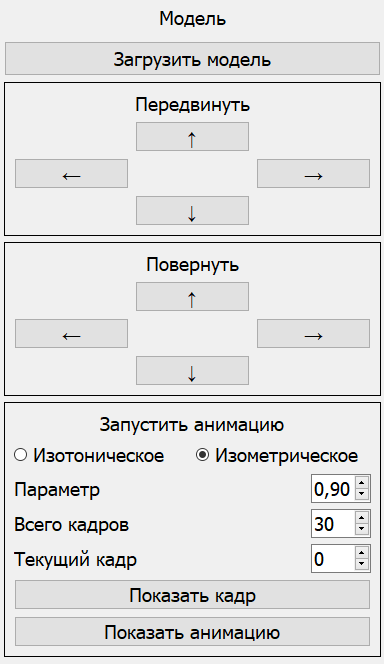
\includegraphics[width=0.4\linewidth]{images/models}
	\caption{Блок взаимодействия с моделями}
	\label{fig:models}
\end{figure}



\section{Вывод}
\label{sec:conc_impl}
В данном разделе были представлены средства, используемые для реализации выбранных алгоритмов, приведены листинги основных классов и функций. Также был рассмотрен реализованный интерфейс программы, модули и диаграмма классов.

%%%% mode: latex
%%%% TeX-master: "rpz"
%%%% End:
                                                                                                                                                 